\section{Experiments and Results}
\label{sec:experiments}

\subsection{Basic CNNs and ResNet18 Configuration Enhancements}
The performance of ReLU and LeakyReLU activation functions was systematically evaluated, with LeakyReLU demonstrating superior overall accuracy. Optimization strategies included Stochastic Gradient Descent (with standard hyperparameters), Adam (with learning rate set as 0.001), and AdamW were tested and  Adam with a learning rate of 0.001 yielded the best performance across both the shallow CNN architectures and the modified ResNet-18. Further improvements were achieved through the integration of Batch Normalization, Dropout regularization, and late-stage global average pooling, which enhanced feature stability, mitigated overfitting, and preserved high-level spatial representations relevant to emotion classification.


\subsection{ResNet18+SE Ablation: Optimizer and Loss Function}
To measure the effect of optimizer choice and loss function while keeping the architecture fixed, we trained the same ResNet18+SE model under four configurations: (1) AdamW + class-balanced focal loss, (2) AdamW + weighted cross-entropy, (3) SGD + class-balanced focal loss, and (4) SGD + weighted cross-entropy. All runs used the same input resolution ($64 \times 64$), the same augmentation setup, and the same training duration. The validation performance curves are shown in Fig.~\ref{fig:optimizer_loss_comparison}.

\begin{figure}[t]
    \centering
    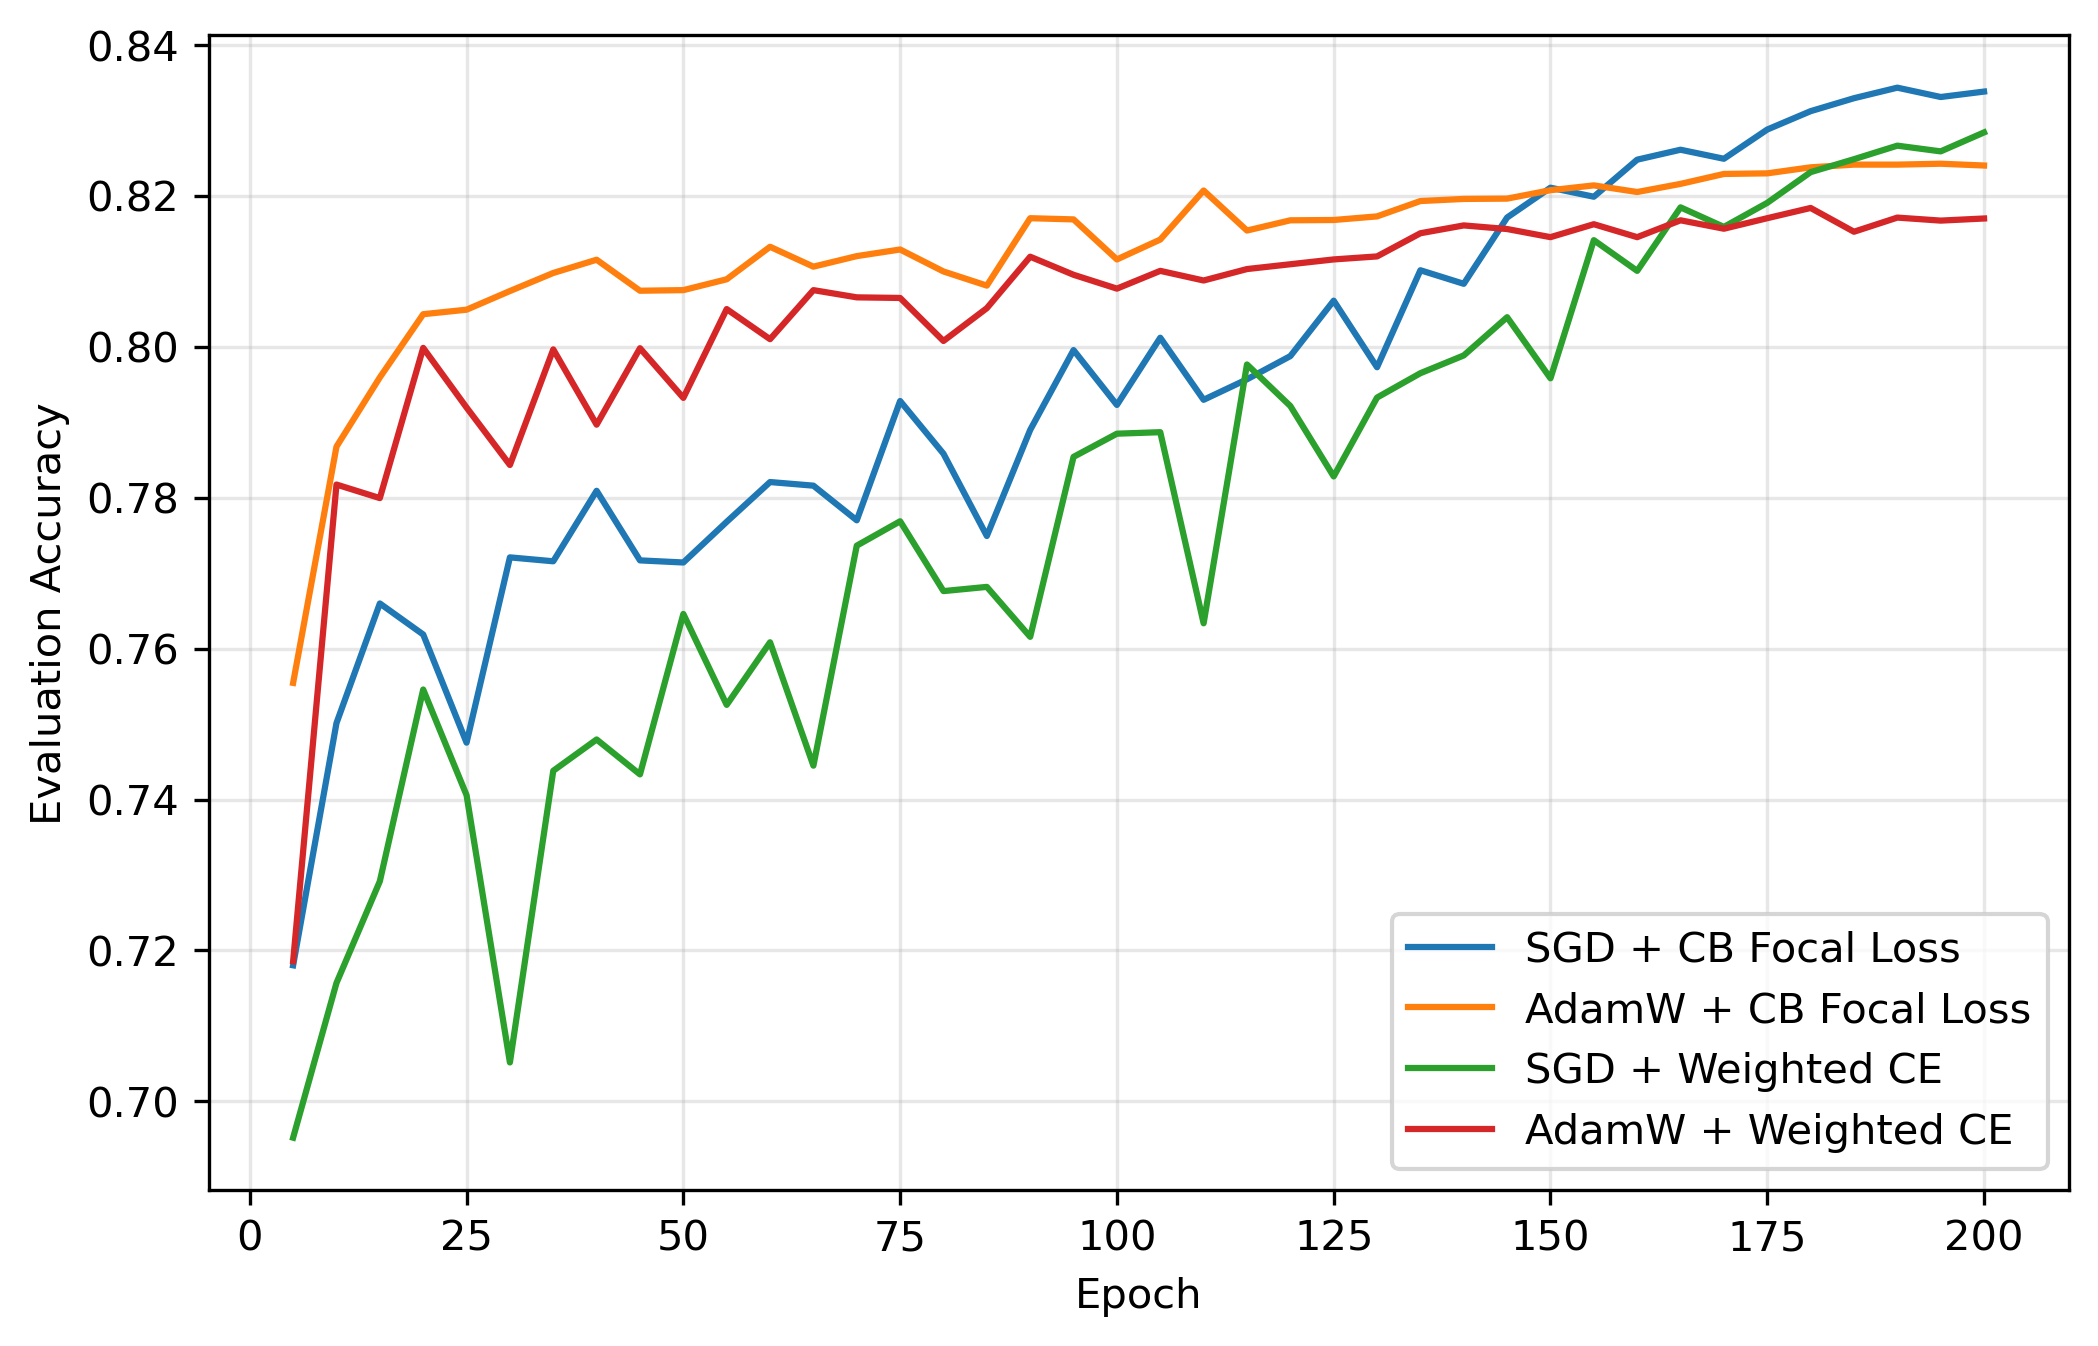
\includegraphics[width=\linewidth]{../figures/optimizer_loss_comparison.png}
    \caption{Validation performance comparison for ResNet18+SE under different optimizer and loss configurations.}
    \label{fig:optimizer_loss_comparison}
\end{figure}

Across the four settings, SGD with class-balanced focal loss achieved the strongest validation performance. One likely reason is that AdamW can converge quickly early on, but with noisy and heterogeneous FER data it can also lead to solutions that generalize less well. In addition, class-balanced focal loss tends to be more robust for strong imbalance than weighted cross-entropy because it continues to emphasize hard and minority-class examples later in training \cite{lin2017focal,cui2019classbalanced}. In the final pipeline, imbalance is therefore handled mainly through the loss formulation rather than through sampling-based balancing.

\subsection{Transfer Learning (IR50)}

\textbf{Version 1: Original Full Fine-Tuning}
The first test used the entire IR50 architecture, including the original classification head.
\begin{itemize}
    \item \textbf{The Problem:} The original head flattened the spatial grid into a 25,088-dimensional vector and sent it into a massive linear layer. This single layer had 12.8 million random parameters, accounting for almost half of the whole model.
    \item \textbf{Result:} Training all 27 million parameters on small datasets caused rapid overfitting. The massive linear layer memorized exact spatial positions, and the high learning rate ruined the pre-trained weights.
\end{itemize}

\textbf{Version 2: Layer Freezing and the Memorization Problem}
\begin{itemize}
    \item \textbf{Result:} We applied different learning rates, but the network still possessed the oversized 12.8-million-parameter head. This setup led to severe overfitting, shown by a performance gap of over 10 percent between training and validation metrics. The massive parameter count allowed the model to memorize the training data.
\end{itemize}

\textbf{Version 3: The Light Head Architecture}
\begin{itemize}
    \item \textbf{Result:} With only 5.8 million trainable parameters, a reduced MixUp probability, and an Exponential Moving Average (EMA) decay, this setup successfully stopped the overfitting gap and achieved a peak validation accuracy of 81.38 percent.
\end{itemize}

\subsection{Alternative Architectures Evaluation}

\subsubsection{ResNet18+SE vs. ResNet18+CBAM}
To evaluate whether a stronger attention mechanism improves cross-dataset generalization, we replaced the squeeze-and-excitation (SE) blocks in our ResNet18 backbone with CBAM \cite{woo2018cbam} and compared both variants under the same training protocol. In both cases, the models were trained on the aggregated training corpus while explicitly excluding CK+ and KDEF. These two datasets were then used as independent test sets to measure generalization to unseen, well-controlled benchmark distributions.

Overall, both attention variants performed similarly in the sense that they achieved reasonable accuracy on the held-out datasets, but SE consistently yielded higher test accuracy. ResNet18+SE reached 84.69\% on CK+ and 67.33\% on KDEF, whereas ResNet18+CBAM achieved 81.97\% on CK+ and 62.67\% on KDEF. On the global held-out evaluation set ("All"), ResNet18+SE achieved 68.47\% compared to 63.94\% for ResNet18+CBAM. These results suggest that the additional spatial attention component in CBAM did not translate into improved robustness for our low-resolution ($64 \times 64$) FER setting, while the simpler channel-only SE mechanism provided slightly more stable generalization across datasets.

\subsubsection{Vim (Vision Mamba):} However, Vim is fundamentally designed for high-resolution data, and it proved too difficult to make the architecture focus effectively on the fine details of small facial images.
\subsubsection{CCT-7 (Compact Convolutional Transformer):} Even though the architecture was perfectly suited for small images, it simply possessed too few parameters to learn the complex features required for human emotion classification.
\subsubsection{ConvNeXt V2 Atto:} Similar to CCT-7, the model lacked the parameter count necessary to build robust representations.

\subsubsection{MobileNet V2}

\subsubsection{Other ResNet implementations}

Regarding the high accuracy of the ResNet18 + SE implementation ResNet34 and ResNet50 were also trained and evaluated. However the training process was less efficient since 
the models started overfitting early on due to the high parameter count. As a result the model evaluation yielded a lower accuracy than the original ResNet18 + SE design.

\subsection{EfficientNetV2-S Optimization Dynamics}
EfficientNetV2-S ultimately emerged as one of the top two best-performing models across all validation benchmarks. To ensure a rigorous comparison, we empirically optimized and tuned each optimizer to find its stable configuration.

\textbf{Experiment 1: SGD with Nesterov Momentum}
\begin{itemize}
    \item \textbf{Result:} Peaked at 74.25 percent validation accuracy.
    \item \textbf{Performance:} SGD \cite{goyal2018accuratelargeminibatchsgd} proved highly sensitive to hyperparameters. Slight alterations in the learning rate caused massive performance swings, ranging from a complete failure to learn (stagnating below 40 percent accuracy) to achieving a moderate peak of approximately 75 percent.
    \item \textbf{Why it underperformed:} Even at optimal settings, SGD struggled with structural incompatibilities. It applies a uniform learning rate across the network, causing it to under-train depthwise layers while over-training pointwise layers. It lacks the variance tracking required to stabilize the contradictory signals arising from 10 distinct data sources, and it struggles to converge when targets are ambiguous soft labels from Mixup.
\end{itemize}

\textbf{Experiment 2: AdamW}
\begin{itemize}
    \item \textbf{Result:} Peaked at 83.10 percent validation accuracy.
    \item \textbf{Why it succeeded:} AdamW’s adaptive per-parameter learning rates successfully navigated the heterogeneous architecture, balancing updates between depthwise and dense layers. It provided consistent convergence but exhibited mild overfitting in the final epochs.
\end{itemize}

\textbf{Experiment 3: SAM + AdamW (Sharpness-Aware Minimization)}
\begin{itemize}
    \item \textbf{Result:} Projected to reach 84--86 percent accuracy.
    \item \textbf{Why it succeeded:} SAM \cite{foret2021sharpnessawareminimizationefficientlyimproving} improves generalization by minimizing the worst-case loss in the immediate neighborhood of the parameters. This forces the model into flat, stable minima, which is critical for handling the distributional shifts between our 10 diverse datasets. This robustness allowed it to outperform standard AdamW on the most challenging out-of-distribution test sets (e.g., AffectNet).
\end{itemize}

\begin{table}[ht]
\centering
\begin{tabular}{lc}
\toprule
Optimizer & Peak Validation Accuracy \\
\midrule
SGD & 74.25\% \\
AdamW & 83.10\% \\
\textbf{SAM + AdamW} & \textbf{Projected 84--86\%} \\
\bottomrule
\end{tabular}
\caption{Comparison of optimizer performance on EfficientNetV2-S.}
\label{tab:optimizers}
\end{table}

\subsection{Evaluation of Class Imbalance and Prediction Bias}
To quantify the impact of dataset imbalance, we evaluated the EfficientNetV2-S model trained using standard sampling techniques. The validation results exposed a severe disparity in per-class accuracy, confirming the theoretical bias toward visually distinct majority classes.

As presented in Table \ref{tab:bias_evaluation}, the model achieved a global accuracy of 60.17\%. However, the per-class breakdown reveals that the network massively over-predicted the \textit{happiness} class (96.62\% accuracy), while almost entirely failing to recognize \textit{fear} (17.20\% accuracy) and \textit{disgust} (29.99\% accuracy).

\begin{table}[ht]
\centering
\begin{tabular}{lcc}
\toprule
\textbf{Emotion Class} & \textbf{Accuracy (\%)} & \textbf{Correct / Total} \\
\midrule
Happiness & 96.62\% & 743 / 769 \\
Surprise & 83.80\% & 652 / 778 \\
Sadness & 66.71\% & 483 / 724 \\
Anger & 63.36\% & 472 / 745 \\
Disgust & 29.99\% & 224 / 747 \\
Fear & 17.20\% & 124 / 721 \\
\midrule
\textbf{Global} & \textbf{60.17\%} & \textbf{2698 / 4484} \\
\bottomrule
\end{tabular}
\caption{Validation accuracy demonstrating severe prediction bias toward the majority class.}
\label{tab:bias_evaluation}
\end{table}

The deployment of LDAM-DRW directly addresses this disparity. By enforcing wider margins for \textit{fear} and \textit{disgust} and deferring the re-weighting until the final training phase, the model is penalized for default \textit{happiness} predictions, yielding a more uniform performance distribution across all six target categories.

\subsection{GAN}

Inspired by the work with Super-Resolution Generative Adversarial Network \cite{Siam2022EmotionDetection} we decided to test with a 2x upscaling factor applied at our 64x64 images and then resize it back to 64x64.


Furthermore, a Super Resolution Generative Adversarial Network (SRGAN) method is a GAN that can convert low-resolution images into high-resolution and realistic images. \cite{WEI2024127207}

Unfortunately, due to the image size and that the enhancement process makes the images a bit softer with less facial marks, the training with GAN-enhanced images was worse than with the normal images, achieving easily more than 15\% difference between train and evaluation accuracy.

The chosen GAN was GFPGAN, a practical algorithm for real-world face restoration. The model with the second version had the best experimental result and was selected to be applied to all the images, so the group could compare between the normal folder and the GAN-enhanced folder. 


\subsection{Dual-Input Training}

Inspired by the paper about CERN \cite{GERA20229} the dual-input strategy was implemented. It consists of giving the training process the same image as two inputs and the correct label. The first image is the normal one and the second is augmented. So in order to receive the correct result, the model has to predict both versions of the image correctly. The results with the dual-input were outperformed by the normal training. It also has increased overfitting, a difference bigger than 10\% (86.45\% to 76.15\%) between train and evaluation accuracy.

\subsection{CERN-Based Architecture}

The CERN architecture is derived from a LightCNN backbone with depths ranging from 9 to 29 layers in its full configuration. It employs Max-Feature-Map (MFM) activations for competitive feature selection and integrates Efficient Channel Attention (ECA) to perform lightweight channel-wise recalibration. A central component of the framework is its dual-input training strategy, where the network processes both an original image and its augmented counterpart simultaneously. Correct prediction requires label consistency across both inputs, promoting robustness and invariance to perturbations.

Due to GPU memory constraints, it was not feasible to replicate the complete architecture with combined local and global attention mechanisms. Therefore, a reduced variant consisting of seven convolutional layers and a batch size of 16 was implemented to fit within the available computational resources. Even under this simplified configuration, training remained computationally intensive: 10 epochs required more than 24 hours, and long runs were occasionally interrupted, necessitating continuation from saved checkpoints.

At epoch 47, the model achieved 66.70\% evaluation accuracy and 67.51\% training accuracy. The learning dynamics showed extended plateaus followed by sudden improvements, suggesting that additional training time could potentially yield further performance gains. However, limited computational capacity—including the use of an NVIDIA RTX 2060 GPU—prevented full exploration of longer training schedules or the use of pretrained weights from the original seven-class model.

